%----------------------------------------------------------------------------------------
%	PACKAGES AND THEMES
%----------------------------------------------------------------------------------------
\documentclass[aspectratio=169,xcolor=dvipsnames]{beamer}

\definecolor{links}{HTML}{2A1B81}
\hypersetup{colorlinks,linkcolor=,urlcolor=links}

\usetheme{Berkeley}

\usepackage{xcolor}
\usepackage{hyperref}
\usepackage{graphicx} % Allows including images
\usepackage{booktabs} % Allows the use of \toprule, \midrule and \bottomrule in tables

%----------------------------------------------------------------------------------------
%	TITLE PAGE
%----------------------------------------------------------------------------------------

% The title
\title[Functional MRI: Part 2 of 2]{Understanding and Interpreting \\Functional Magnetic Resonance Imaging}
\subtitle{Precision Health Boot Camp}

\author[Dr. Alexander Mark Weber] {Alexander Mark Weber}
\institute[UBC] % Your institution may be shorthand to save space
{
    % Your institution for the title page
    Department of Pediatrics, Division of Neurology \\
    University of British Columbia 
    \vskip 3pt
}
\date{12:00 - 2:00 PM \\August 9th, 2022} % Date, can be changed to a custom date


%----------------------------------------------------------------------------------------
%	PRESENTATION SLIDES
%----------------------------------------------------------------------------------------

\begin{document}

\begin{frame}
    % Print the title page as the first slide
    \titlepage
\end{frame}

\begin{frame}{Preamble}

\begin{columns}[c]
\column{0.4\textwidth}
\begin{center}
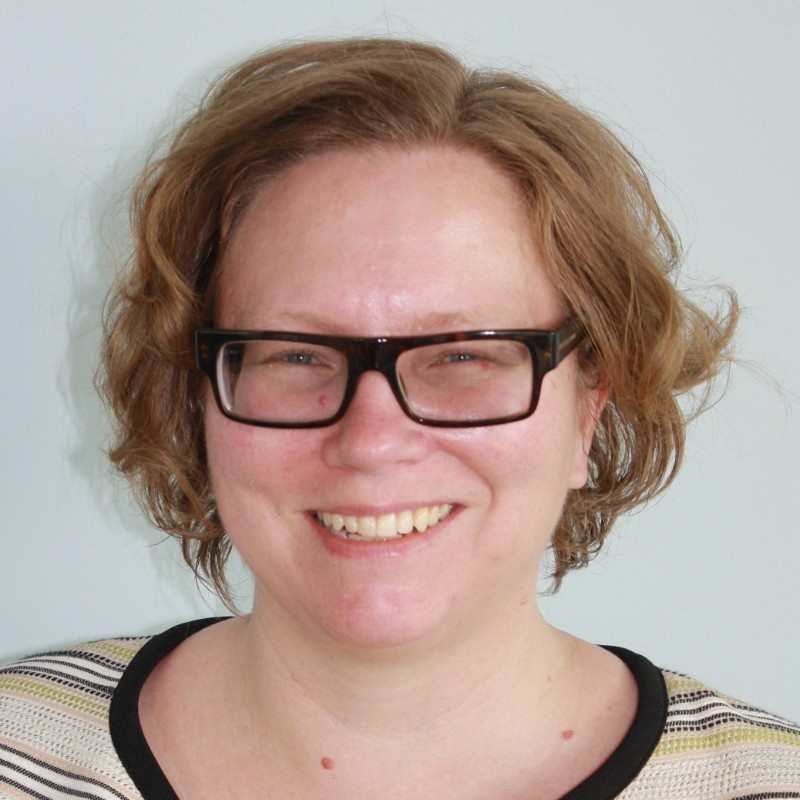
\includegraphics[width=.7\textwidth]{imgs/Lynne}
\end{center}

\column{0.6\textwidth}


\includegraphics[width=.9\textwidth]{imgs/lit6}

\vspace{.2cm}

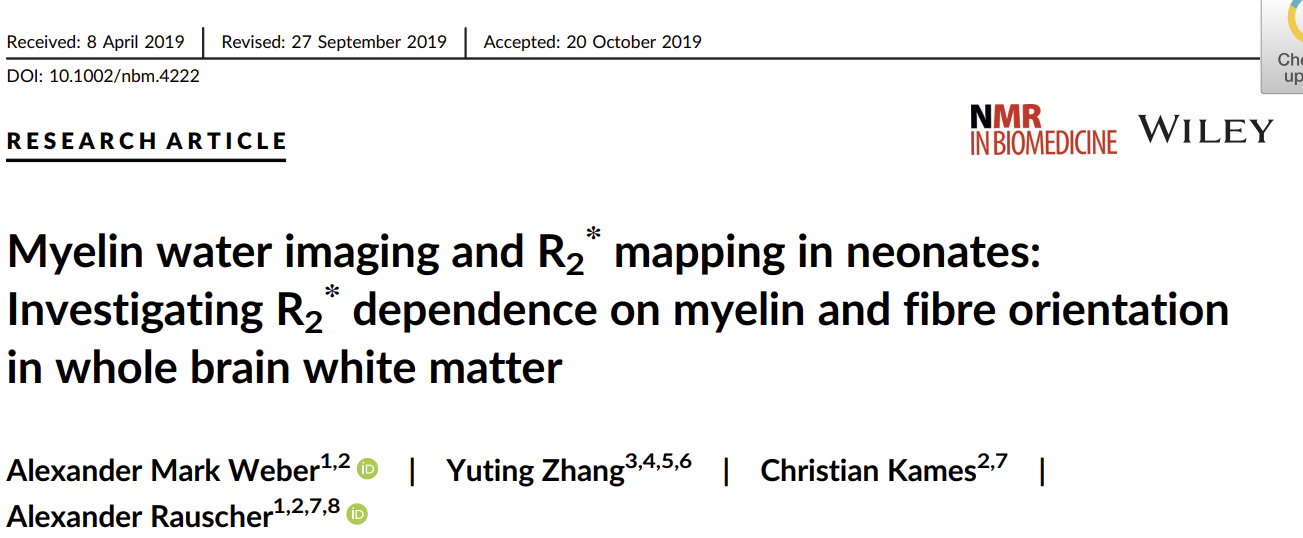
\includegraphics[width=.9\textwidth]{imgs/lit7}


\end{columns}
\end{frame}

\begin{frame}{Overview}
    % Throughout your presentation, if you choose to use \section{} and \subsection{} commands, these will automatically be printed on this slide as an overview of your presentation
    \tableofcontents
\end{frame}

%------------------------------------------------
\section{Housekeeping}
%------------------------------------------------

\begin{frame}{Land Acknowledgement}

I would like to acknowledge that we are gathered today on the traditional, ancestral, and unceded territory of the Musqueam people.

\vspace{0.2cm}
\begin{center}
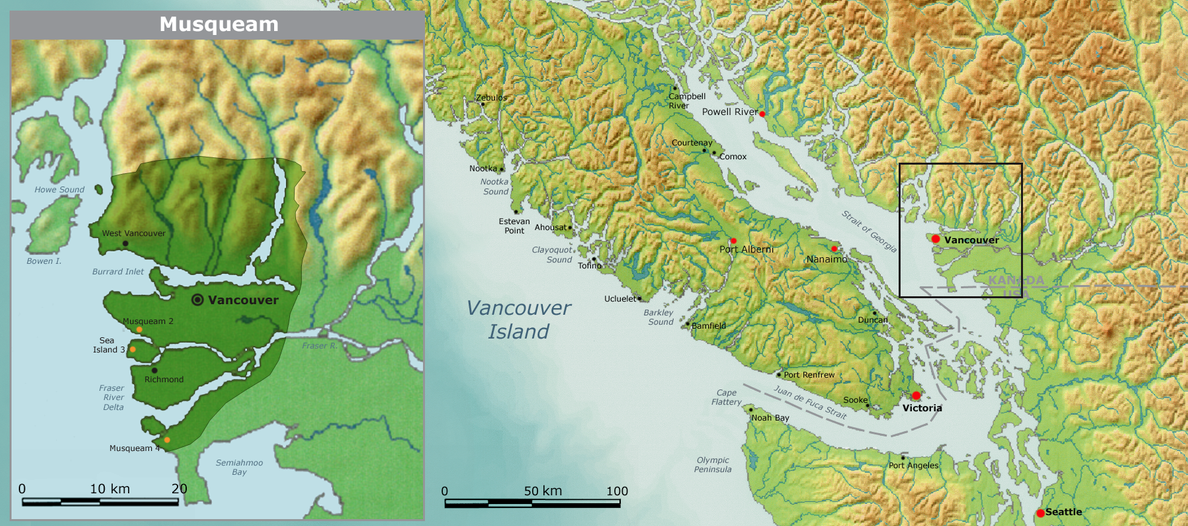
\includegraphics[width=.9\textwidth]{imgs/musqueam}
\end{center}

\end{frame}

%------------------------------------------------

\begin{frame}{Copyright Information}

\begin{columns}[c]
\column{0.5\textwidth}
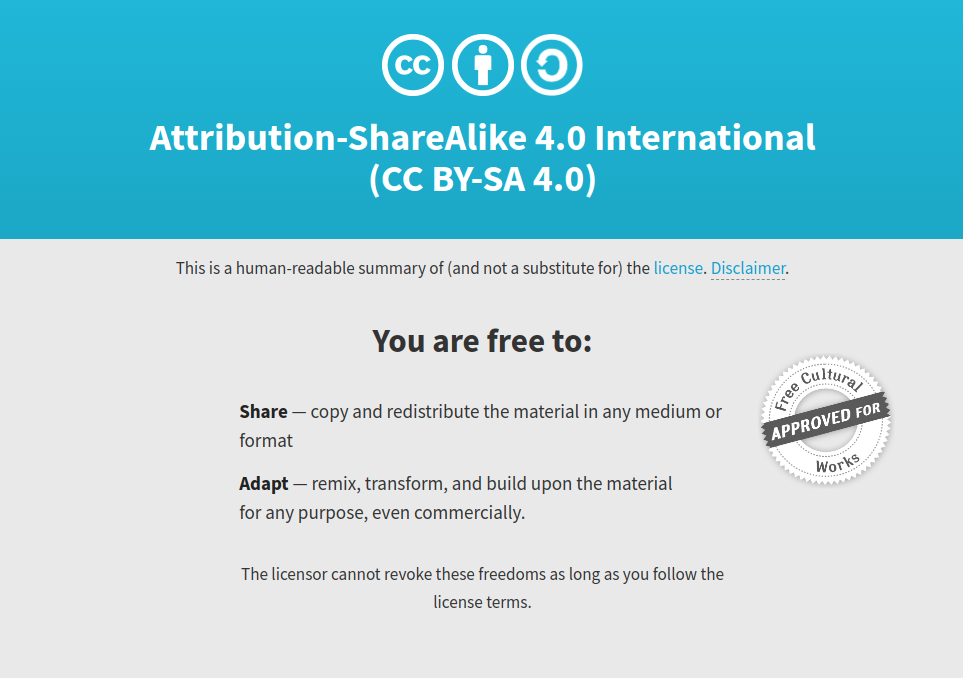
\includegraphics[width=1\textwidth]{imgs/cc}
\column{0.5\textwidth}
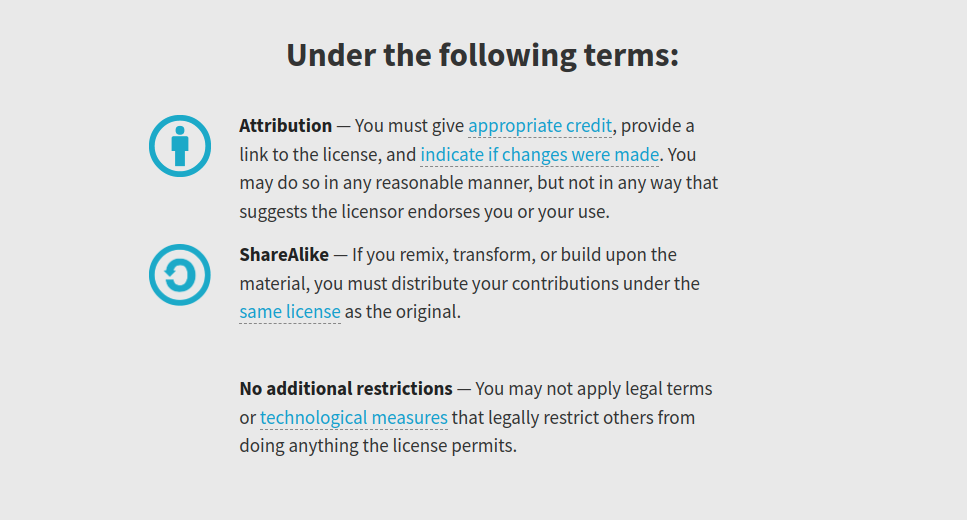
\includegraphics[width=1\textwidth]{imgs/cc2}
\end{columns}

\vspace{.5cm}
Read more here: \url{https://creativecommons.org/licenses/by-sa/4.0/}

\end{frame}

%------------------------------------------------
\section{Freesurfer and DTI Overview}
%------------------------------------------------

\begin{frame}{Freesurfer and DTI Overview}
\begin{columns}[c]
\column<1->{0.45\textwidth}
\vspace{-.4cm}

\begin{center}
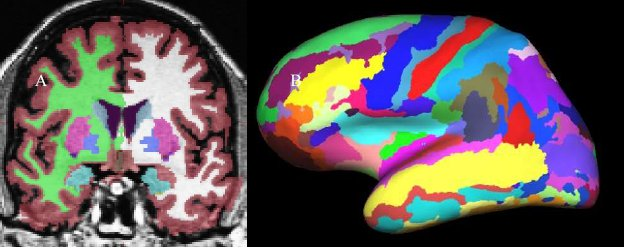
\includegraphics[width=.5\textwidth]{imgs/FSanalysisPipelineFig4}

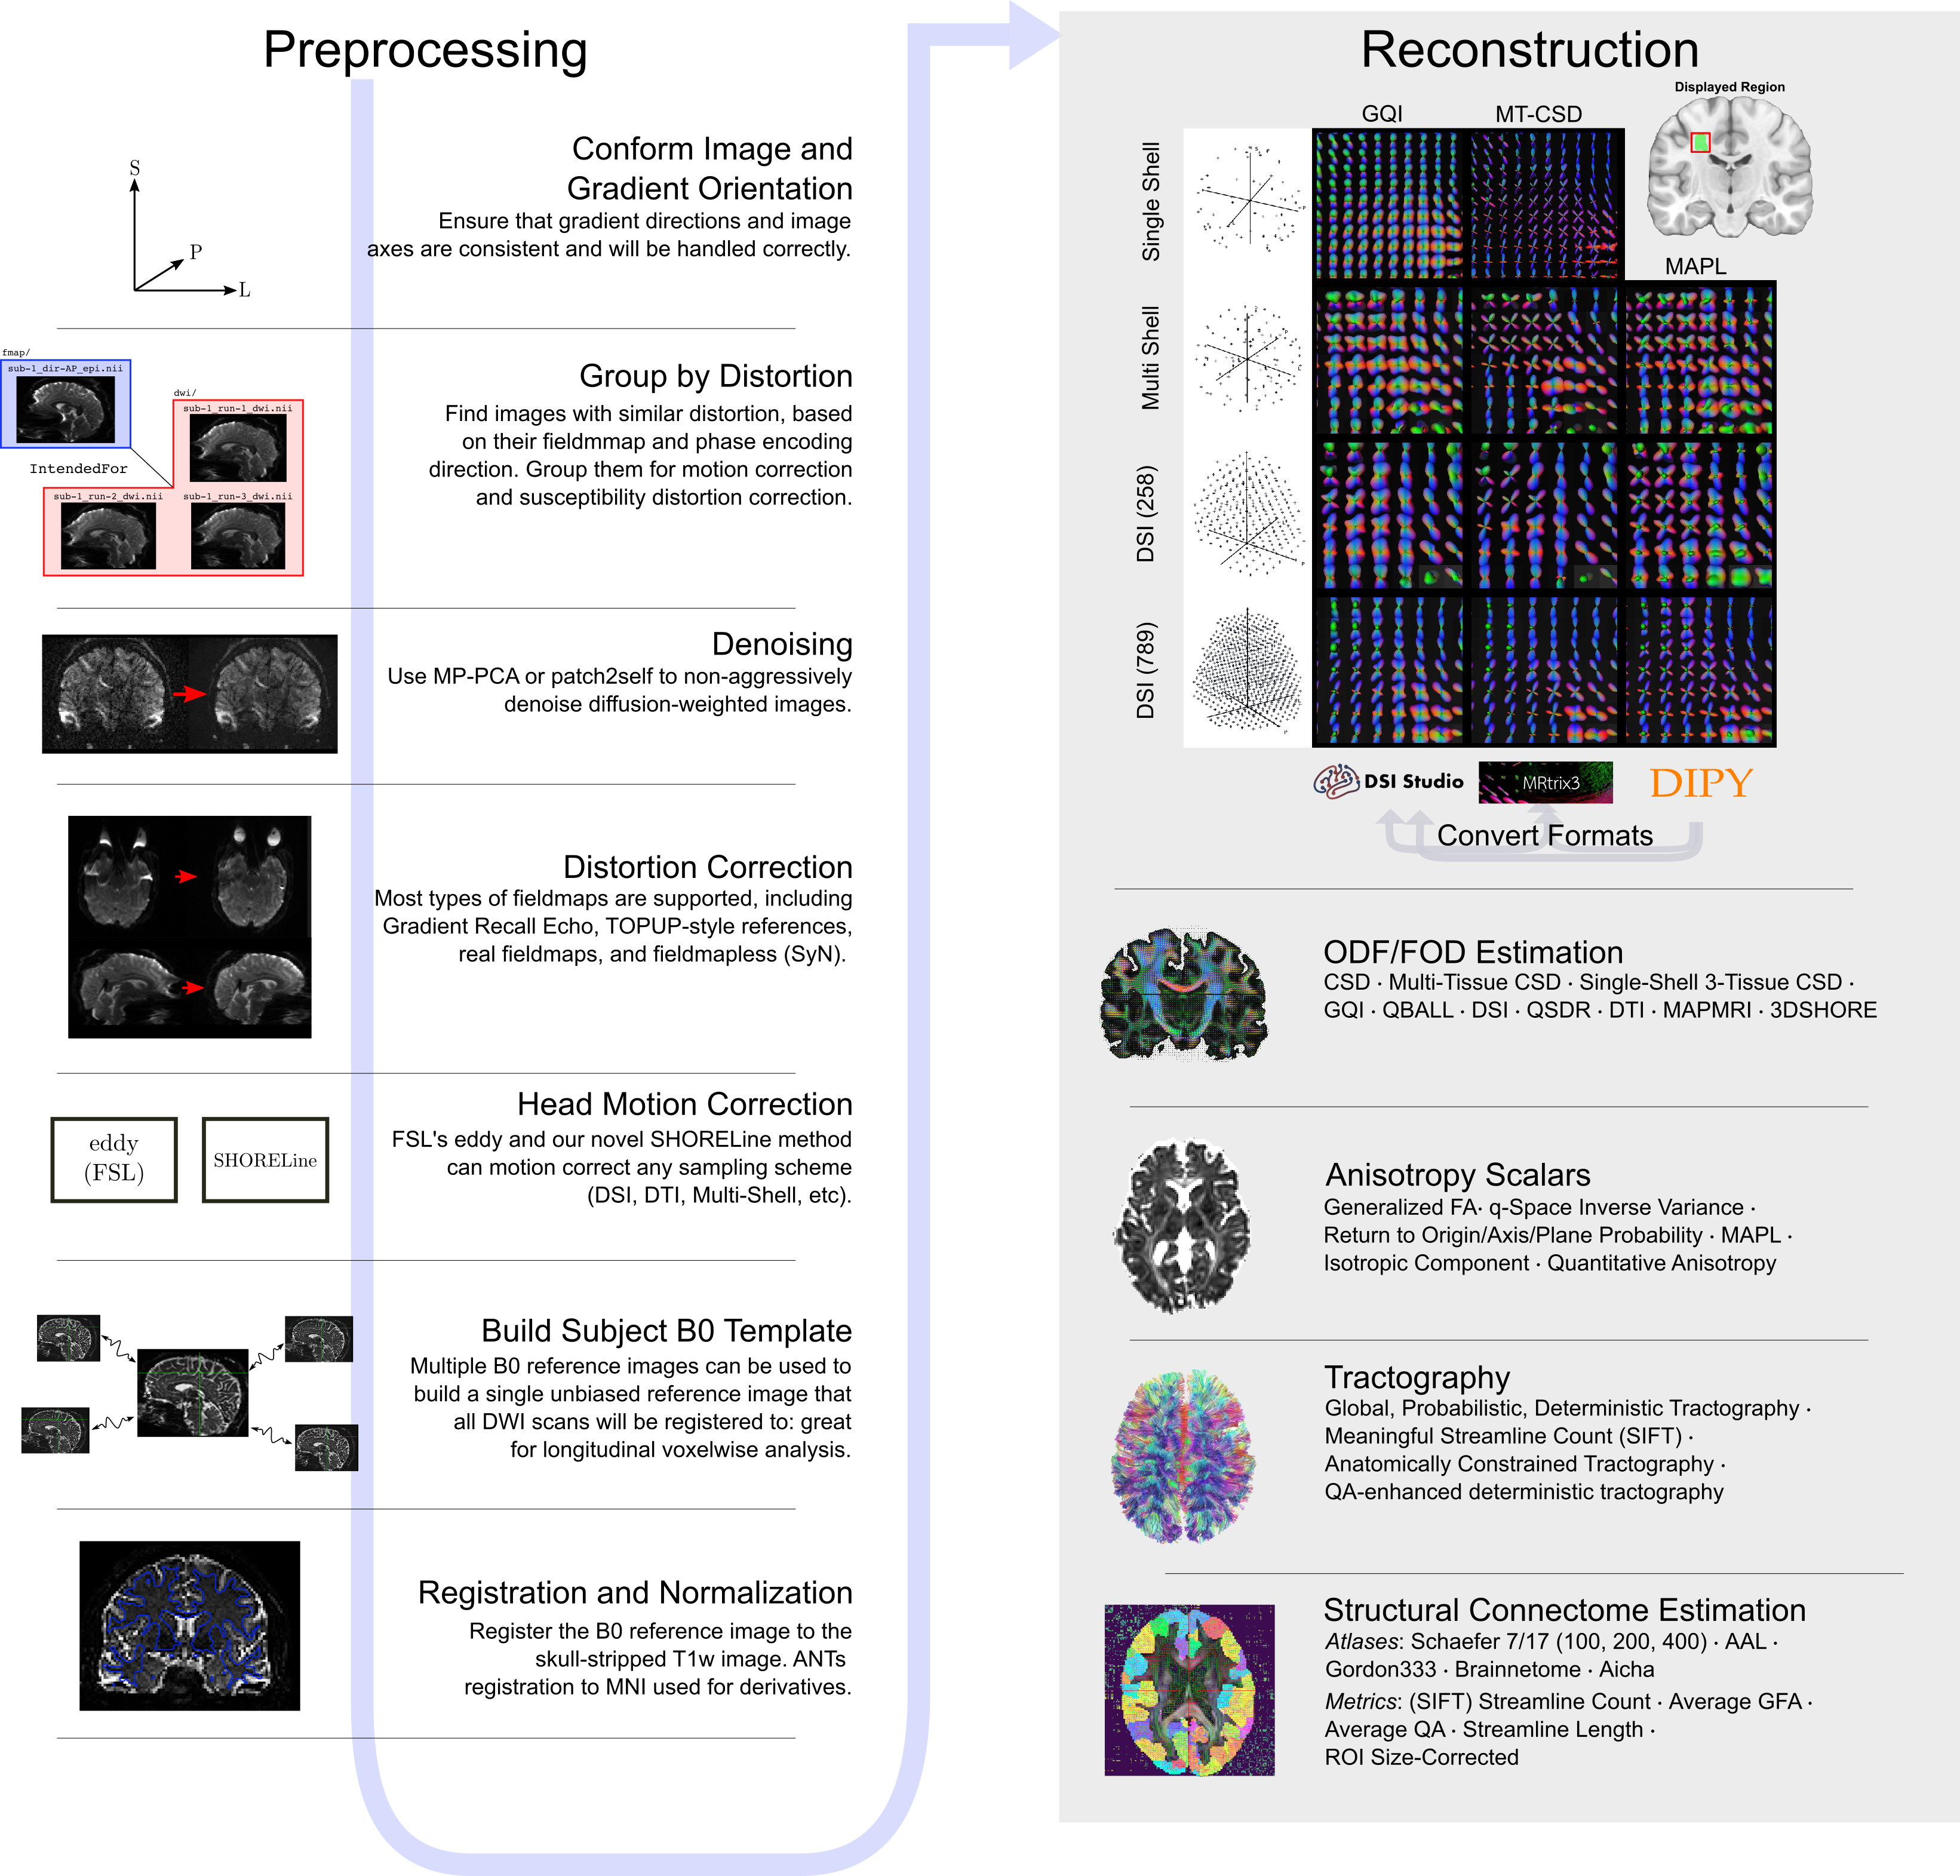
\includegraphics[width=1\textwidth]{imgs/qsiprep_workflow_full}
\tiny{surfer.nmr.mgh.harvard.edu/; }
\end{center}

\column<2->{0.55\textwidth}
Lecture:
\begin{itemize}
\item T$_{1}$ and T$_{2}$ weighted imaging
\end{itemize}

Tutorial:
\begin{itemize}
\item Freesurfer
\end{itemize}

Lecture:
\begin{itemize}
\item DTI Physics
\end{itemize}

Tutorial:
\begin{itemize}
\item DTI preprocessing using \texttt{qsiprep}
\end{itemize}
\end{columns}

\end{frame}

%------------------------------------------------
\section{Learning Objectives}
%------------------------------------------------

\begin{frame}
At the end of this session, students will be able to:
\begin{itemize}
\item Describe the difference between T$_{1}$ and T$_{2}$ weighted images
\item How to run \texttt{Freesurfer} on Sockeye
\item Describe why water diffusion in the brain can help us understand white matter structure
\item Describe how MRIs detect diffusion in different directions
\item How to run \texttt{qsiprep} to preprocess DWI on Sockeye
\end{itemize}
\end{frame}

%------------------------------------------------
\section{MRI Physics: T$_{1}$ and T$_{2}$ Weighted Imaging}
%------------------------------------------------

\begin{frame}{T$_{1}$ and T$_{2}$ Overview}
\begin{columns}[c]
\column{0.5\textwidth}
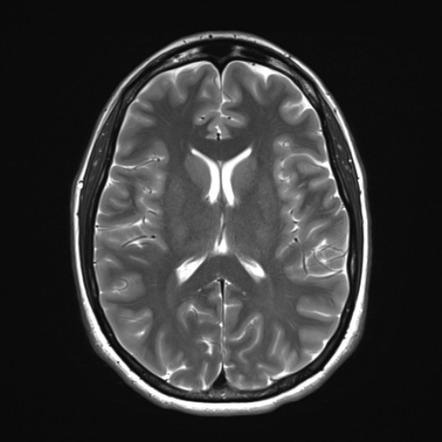
\includegraphics[width=1\textwidth]{imgs/t2brain}
\column{0.5\textwidth}
T$_{2}$-weighted scan
\begin{itemize}
\item Water is bright
\item A mix of water/tissue is less bright (grey matter)
\item Fatty tissue is dark (white matter)
\end{itemize}
\end{columns}

\end{frame}

%------------------------------------------------

\begin{frame}{T$_{1}$ and T$_{2}$ Overview}
\begin{columns}[c]
\column{0.5\textwidth}
\begin{center}
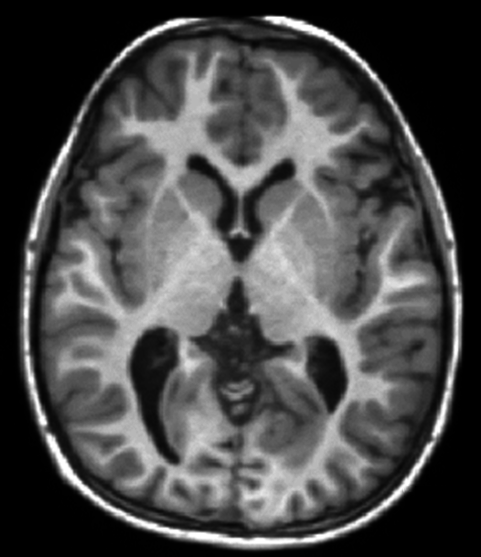
\includegraphics[width=.8\textwidth]{imgs/t1brain}
\end{center}

\column{0.5\textwidth}
T$_{1}$-weighted scan
\begin{itemize}
\item Fatty tissue is bright (white matter)
\item A mix of water/tissue is less bright (grey matter)
\item Water is dark
\end{itemize}
\end{columns}

\end{frame}

%------------------------------------------------

\begin{frame}{T$_{1}$ and T$_{2}$ Overview}
\begin{columns}[c]
\column{0.5\textwidth}
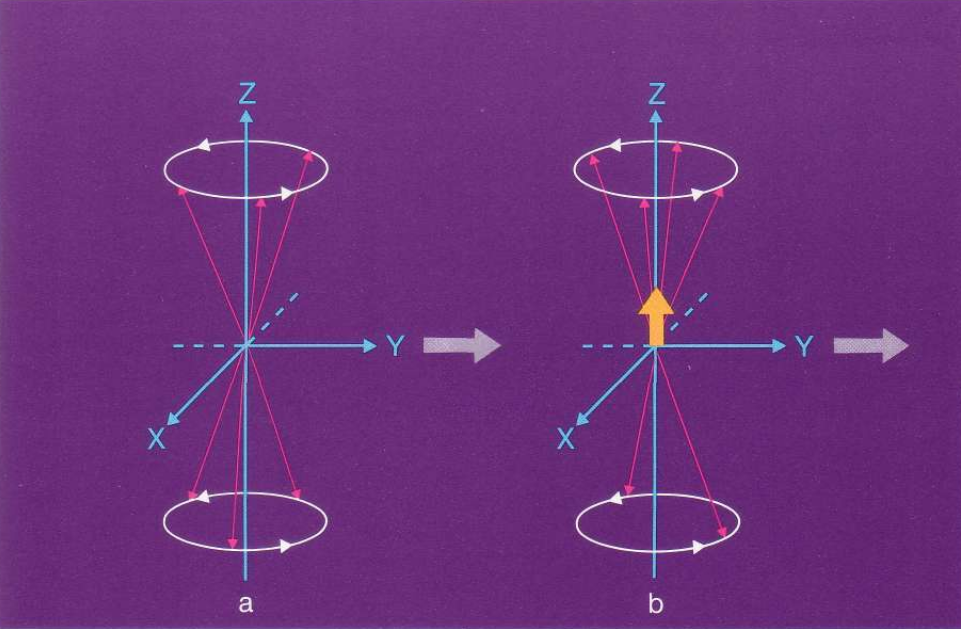
\includegraphics[width=1\textwidth]{imgs/longrelax}
\column{0.5\textwidth}
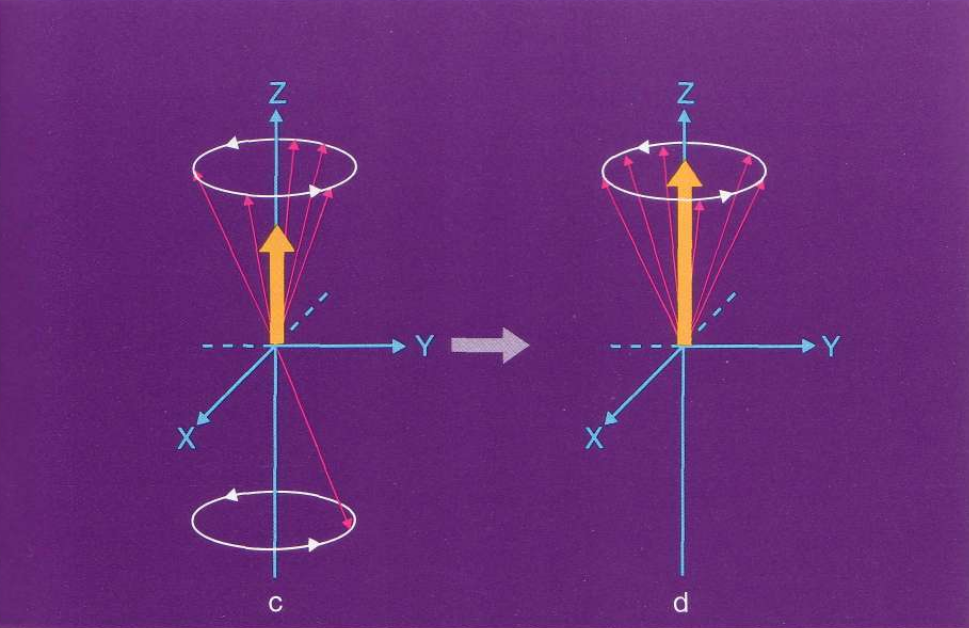
\includegraphics[width=1\textwidth]{imgs/longrelax2}
\end{columns}

\end{frame}

%------------------------------------------------

\begin{frame}{T$_{1}$ and T$_{2}$ Overview}
    \begin{block}{T1 relaxation}
        Also known as spin-lattice or longitudinal relaxation: it is a time measure of the rate of recovery caused by spin-lattice interactions
    \end{block}
\begin{center}
\includegraphics[width=.75\textwidth]{imgs/T1recoverycurve}

\end{center}
\end{frame}

%------------------------------------------------

\begin{frame}{T$_{1}$ and T$_{2}$ Overview}
\begin{columns}[c]
\column{0.6\textwidth}
\begin{center}
\includegraphics<1->[width=1\textwidth]{imgs/t1t2}
\end{center}

\column{0.4\textwidth}
\begin{center}
\includegraphics<2->[width=.8\textwidth]{imgs/t1brain}
\end{center}
\end{columns}

\end{frame}


%------------------------------------------------
\section{Freesurfer Analysis}
%------------------------------------------------

\begin{frame}{Freesurfer}
\begin{center}
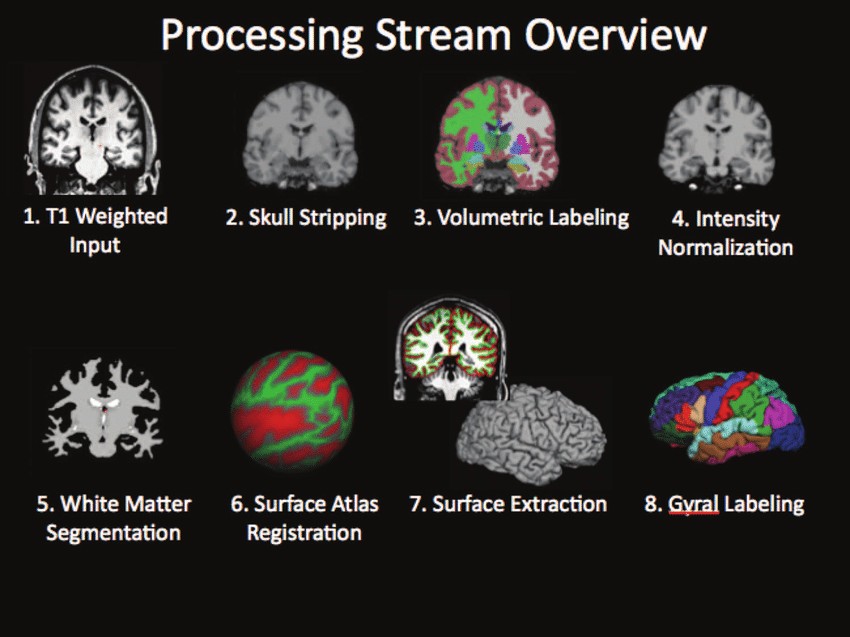
\includegraphics[width=.7\textwidth]{imgs/fspipeline}

\end{center}
\end{frame}

%------------------------------------------------
\section{Freesurfer Tutorial}
%------------------------------------------------

\begin{frame}{Sockeye}

\end{frame}

%------------------------------------------------
\section{MRI Physics: DWI}
%------------------------------------------------

\begin{frame}{Diffusion Weighted Imaging}
\begin{columns}
\column{0.5\textwidth}
\begin{block}<1->{Diffusion Weighted Imaging}
\begin{itemize}
\item diffusion-weighted imaging is an MRI technique based on the tissue \textbf{water diffusion rate}
\item It allows for very sensitive probing of water movements within the architecture of the tissues
\end{itemize}
\end{block}

\begin{block}<2->{Brownian Motion}
random motion of particles suspended in a medium
\end{block}

\column{0.5\textwidth}
\includegraphics<3->[width=1\textwidth]{imgs/diffusion}
\onslide<3->
\tiny{McRobbie et al. MRI: From Picture to Proton, 2nd Ed}
\end{columns}
\end{frame}

%------------------------------------------------

\begin{frame}{Diffusion Weighted Imaging}
\begin{center}
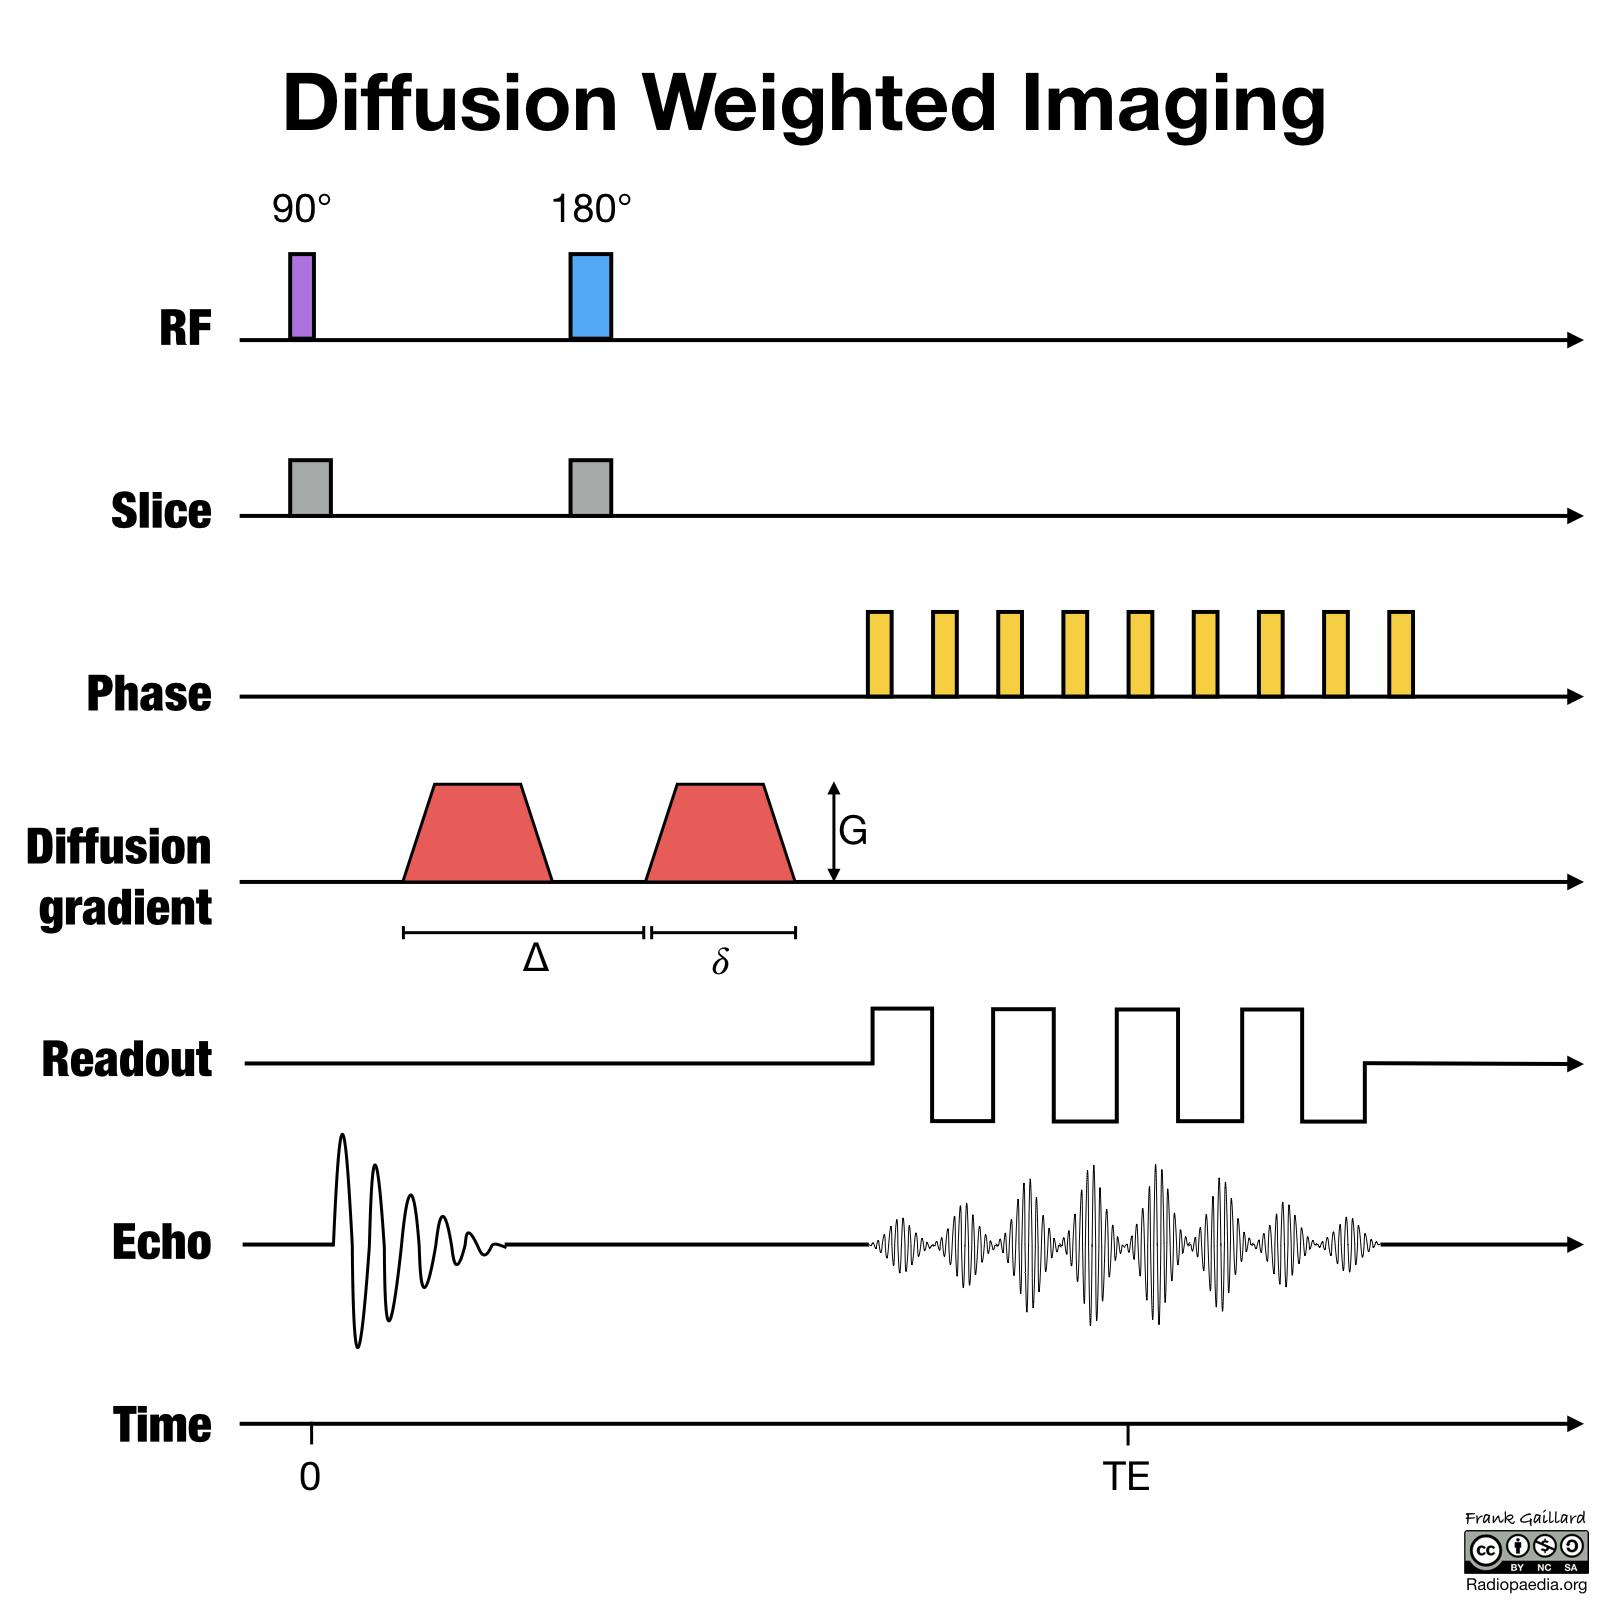
\includegraphics[width=.5\textwidth]{imgs/mri-physics-diagrams-1}

\tiny{Frank Gaillard, Radiopaedia.org}
\end{center}

\end{frame}

%------------------------------------------------

\begin{frame}{Diffusion Weighted Imaging}
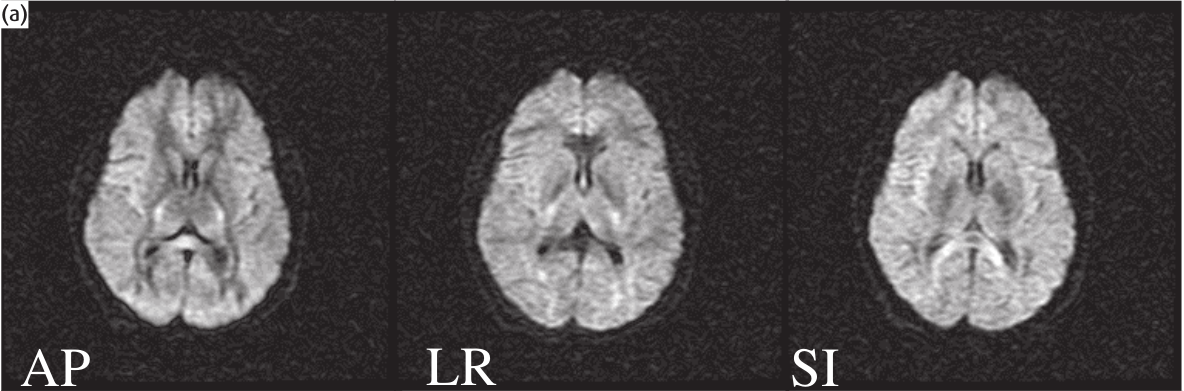
\includegraphics[width=1\textwidth]{imgs/threedirectionsdiffusion}

\tiny{McRobbie et al. MRI: From Picture to Proton, 2nd Ed}
\end{frame}
%------------------------------------------------

\begin{frame}{Diffusion Tensor Imaging}
\begin{columns}
\column{0.5\textwidth}
\begin{center}
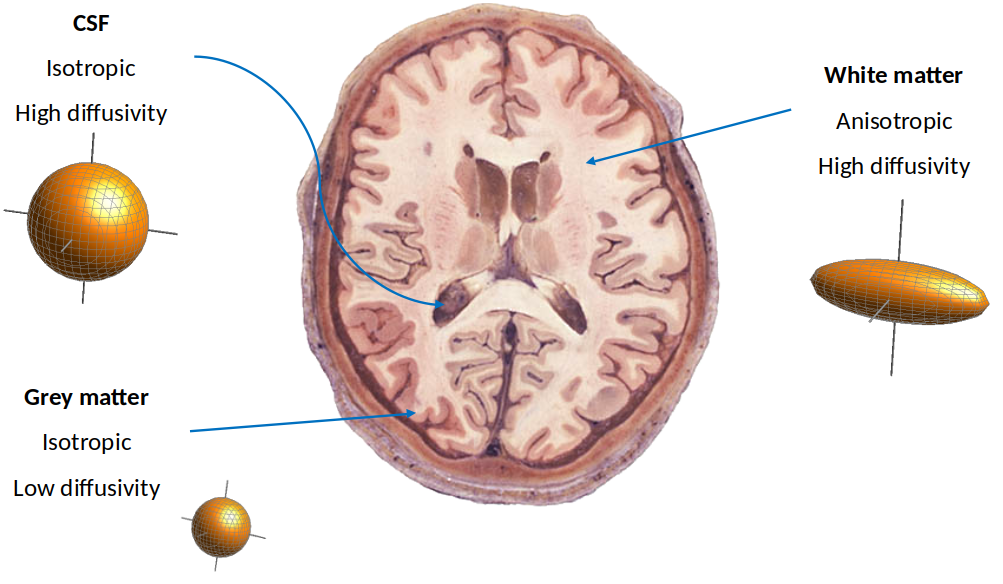
\includegraphics[width=1\textwidth]{imgs/diffusionprinciple}

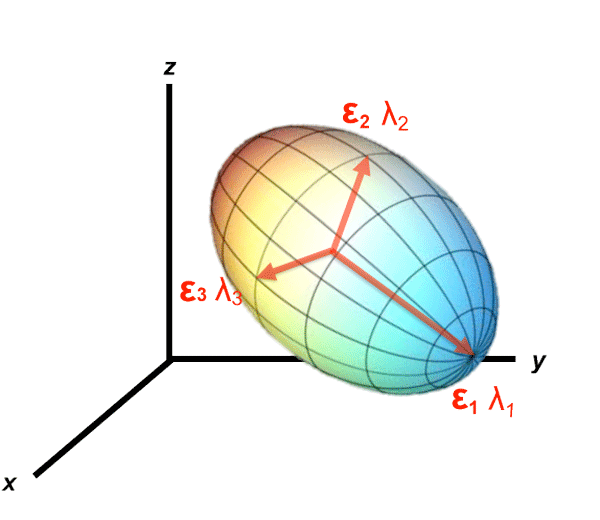
\includegraphics[width=.5\textwidth]{imgs/tensor}
\end{center}

\column{0.5\textwidth}

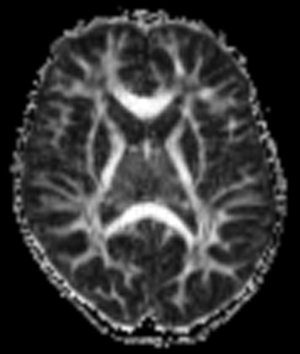
\includegraphics[width=.4\textwidth]{imgs/FA}%
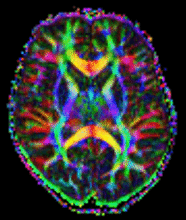
\includegraphics[width=.4\textwidth]{imgs/colorFA}%
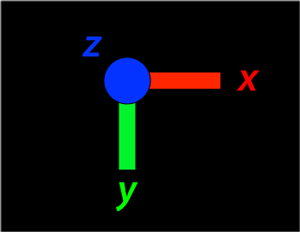
\includegraphics[width=.2\textwidth]{imgs/colormap}

\begin{center}
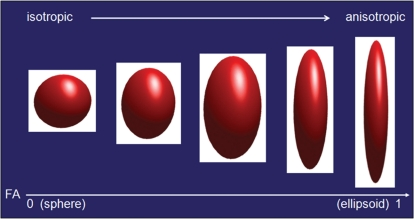
\includegraphics[width=.8\textwidth]{imgs/FAtensors}
\end{center}
\end{columns}
\end{frame}

%------------------------------------------------

\begin{frame}{Tractography}
\begin{columns}
\column{0.5\textwidth}
\begin{center}
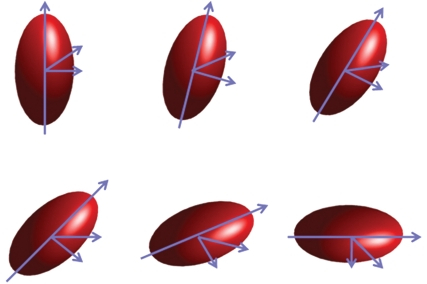
\includegraphics[width=1\textwidth]{imgs/eigvec}
\end{center}

\column{0.5\textwidth}

\begin{center}
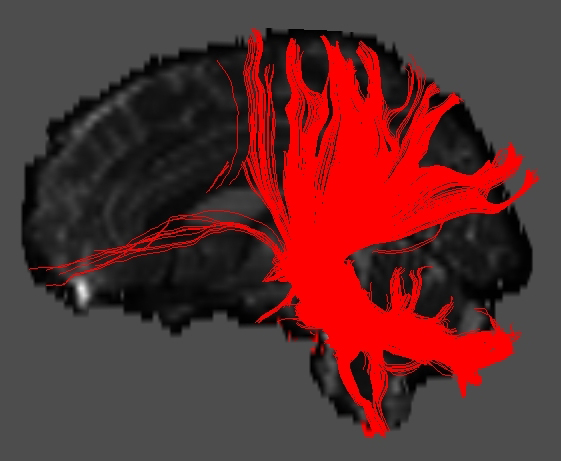
\includegraphics[width=1\textwidth]{imgs/fibretracking}
\end{center}
\end{columns}
\end{frame}

%------------------------------------------------

\begin{frame}{DWI Preprocessing}
\begin{columns}
\column{0.5\textwidth}
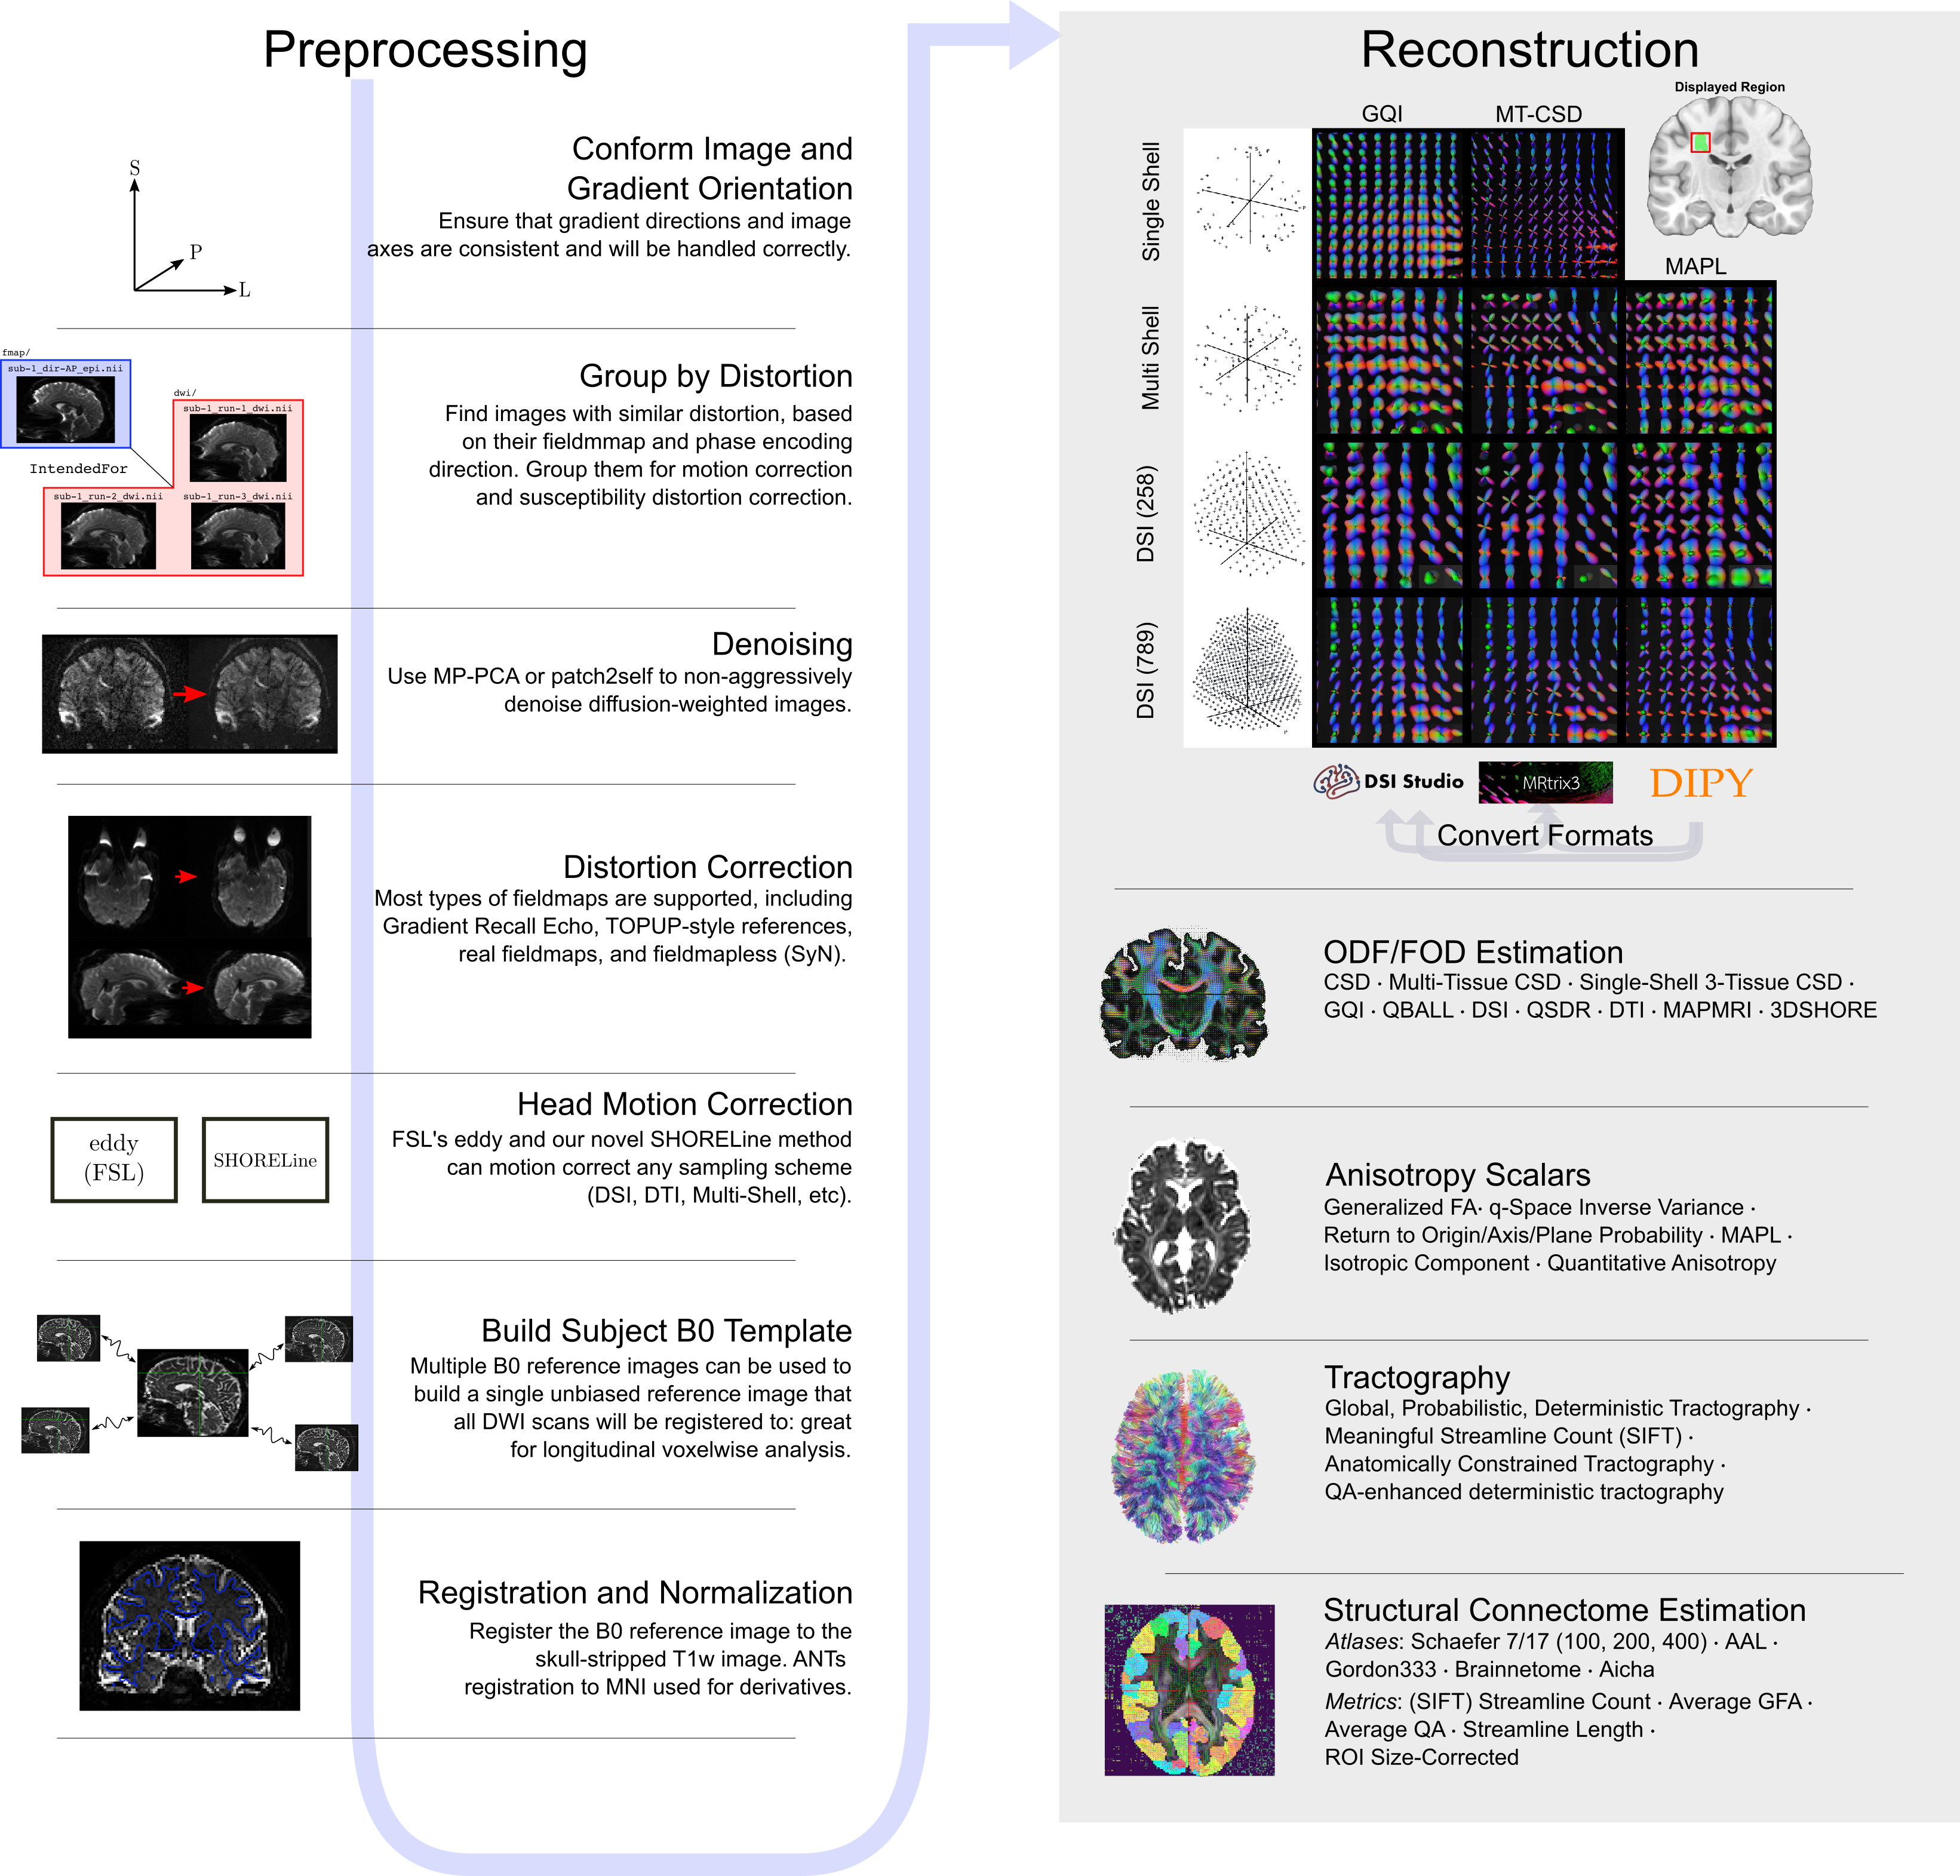
\includegraphics[width=1\textwidth]{imgs/qsiprep_workflow_full}

\column{0.5\textwidth}
\begin{itemize}
\item Brain extraction
\item Head motion correction
\item Eddy current correction
\item Susceptibility distortion
\item Coregistration to T1w images
\item Spatial normalization
\item Data quality checks

\end{itemize}
\end{columns}

\end{frame}

%------------------------------------------------
\section{DWI Tutorial}
%------------------------------------------------

\begin{frame}{Sockeye}

\end{frame}


\end{document}